\documentclass[aspectratio=169]{beamer}
\usetheme{metropolis}           % Use metropolis theme
\metroset{numbering=fraction}
\usepackage{tikz}
\usetikzlibrary{positioning}
\usetikzlibrary{arrows,backgrounds,automata,decorations.shapes,decorations.pathmorphing,decorations.markings,decorations.text,positioning,shapes.geometric}

\tikzstyle{place}=[circle,draw=blue!50,fill=blue!20,thick, inner sep=0pt,minimum size=6mm]
\tikzstyle{transition}=[rectangle,draw=black!50,fill=black!20,thick, inner sep=0pt,minimum size=4mm]

\tikzstyle{block}=[rectangle,draw=black, thick, inner sep=5pt]
\tikzstyle{bullet}=[circle,draw=black, fill=black, thin, inner sep=2pt]

\tikzstyle{pre}=[<-,shorten <=1pt,>=stealth',semithick]
\tikzstyle{post}=[->,shorten >=1pt,>=stealth',semithick]
\tikzstyle{bi}=[<->,shorten >=1pt,shorten <=1pt, >=stealth',semithick]

\tikzstyle{mut}=[-,>=stealth',semithick]

\tikzstyle{treereset}=[dashed,->, shorten >=1pt,>=stealth',thin]

\pgfdeclarelayer{edgelayer}
\pgfdeclarelayer{nodelayer}
\pgfsetlayers{edgelayer,nodelayer,main}

\tikzstyle{none}=[inner sep=0pt]
\tikzstyle{rn}=[circle,fill=Red,draw=Black,line width=0.8 pt]
\tikzstyle{gn}=[circle,fill=Lime,draw=Black,line width=0.8 pt]
\tikzstyle{yn}=[circle,fill=Yellow,draw=Black,line width=0.8 pt]
\tikzstyle{empty}=[circle,fill=White,draw=Black]
\tikzstyle{bw} = [rectangle, draw, fill=blue!20, 
    text width=4em, text centered, rounded corners, minimum height=2em]

\usepackage{float}
\usepackage{makecell}
\usepackage{fancyvrb}
\usepackage{listings}
\usepackage[export]{adjustbox}
\usepackage{caption}
\usepackage{alltt}
\title{Lecture 6 \\ Timers, Java Exceptions}
\date{May 19, 2016}
\author{Patrick Lam \\ Jeff Zarnett \\ Michael Giannikouris}
\institute{Department of Electrical and Computer Engineering}
\setbeamertemplate{caption}{\raggedright\insertcaption\par}
\setbeamersize{text margin left=12pt,text margin right=12pt}
\newcommand{\putat}[3]{\begin{picture}(0,0)(0,0)\put(#1,#2){#3}\end{picture}} % just a shorthand

\newenvironment{deflist}
{ \begin{description}
    \setlength{\itemsep}{6pt}
    \setlength{\parskip}{0pt}
    \setlength{\parsep}{0pt}     }
{ \end{description}              } 

\newenvironment{splitslide}
{
\centering
\begin{tabular}{@{}p{0.50\textwidth} | p{0.025\textwidth}@{} p{0.4\textwidth}@{}}
}
{
\end{tabular}
}

\newcounter{tmpnumSlide}
\newcounter{tmpnumNote}

 \newcommand\mnote[1]{%
   \addtocounter{tmpnumSlide}{1}
   \ifdefined\showcues {~\tiny\fbox{\arabic{tmpnumSlide}}}\fi
   \note{\setlength{\parskip}{1ex}\addtocounter{tmpnumNote}{1}\textbf{\Large \arabic{tmpnumNote}:} {#1\par}}}


\begin{document}
\maketitle



\section*{Timers}



\begin{frame}{Applications of Timers}
\Large
Interval Timers --- perform a task occasionally.\\
\begin{itemize}
\item raising alarms
\item polling
\end{itemize}
Watchdog Timers --- reset a stuck system.
~\\[1.5em]
We'll use Java timers to implement these,
and learn the difference between Android and Java timers.
\end{frame}



\section{Interval Timers}



\begin{frame}{Interval Timers}
\Large
Good for recurring tasks.\\[1em]
\vspace{1em}
Typical Embedded System Example: \textbf{Sensor polling} \\
\quad (not on Android --- receive sensor events instead).\\[1em]
\vspace{1em}
The Android Way: {\tt Handler} for interval timers.
\end{frame}



\begin{frame}{Classes Related to Android Handler}
\begin{itemize}
\item \texttt{Handler}: 
\begin{itemize}\item This (Android) class sends and processes objects from a MessageQueue for a specific thread. \end{itemize}
\item \texttt{Runnable}: 
\begin{itemize}
\item This (Java) interface is implemented by a class containing code to be delegated (e.g. to another thread or passed to a queue). \\
\item Contains a single method, \texttt{void run()}\\
\end{itemize}
\end{itemize}
\end{frame}



\begin{frame}[fragile]{Handlers for Infinitely-Recurring Interval Timers}
\begin{Verbatim}
  Handler h = new Handler();
  Runnable r = new Runnable() {
    public void run() {
      // execute the task
      h.postDelayed(this, delayInMS);
    }
  };
  h.postDelayed(r, delayInMS);
\end{Verbatim}
\end{frame}




\begin{frame}[fragile]{Cancelling Tasks}
By the way, you can cancel an upcoming task like this:
\begin{Verbatim}
  h.removeCallbacks(r);
\end{Verbatim}
\end{frame}




\begin{frame}{True Interval Timers}
\large
Handlers run when the thread is available.\\[1em]

True interval timers interrupt the processor.

Can simulate with {\tt java.util.Timer}\footnote{\url{http://steve.odyfamily.com/?p=12}, accessed
  February 3, 2013.} (Java timers). \\[1em]

Callback (code) runs in a different thread:
\begin{itemize}
\item[(+)] more predictable timing;
\item[(--)] can't update UI from other thread.
\end{itemize}
~\\
Generally more overhead for {\tt java.util.Timer}, not great for Android apps.
\vspace{1em}
\end{frame}



\begin{frame}[fragile]{Using a Java Timer}
\begin{columns}
\begin{column}{0.45\textwidth}
\begin{Verbatim}[fontsize=\footnotesize]
  Timer t = new Timer();
  t.schedule(new TimerTask() {
    @Override
    public void run() {
      // do stuff when timer fires
    }
  }, firstDelayMS, repeatIntervalMS);
\end{Verbatim}
\end{column}
\begin{column}{0.05\textwidth}\end{column}
\begin{column}{0.50\textwidth}
\begin{normalsize}
\pause
\vspace{0.5em}
Create an instance of the \texttt{Timer} class. \\
\pause
\vspace{1em}
Provide an instance of the \texttt{TimerTask} class to the Timer via \texttt{schedule()}. \\
\pause
\vspace{1em}
TimerTask implements \texttt{Runnable}, so we override \texttt{run()} with code we want to run when the timer fires. \\
\pause
\vspace{1em}
If you omit repeatIntervalMS, you get a one-shot timer.
\end{normalsize}
\end{column}
\end{columns}
\end{frame}



\begin{frame}[fragile]{Java Timer: Getting Around UI Thread Issues}
In the \texttt{run()} method of \texttt{TimerTask}, call \texttt{runOnUiThread()} and pass a \texttt{Runnable()}. \\
\vspace{0.5em}
Android will pass the Runnable() to the UI thread for execution. \\
\vspace{1em}
\begin{splitslide}

\begin{Verbatim}[fontsize=\footnotesize]
  Timer t = new Timer();
  t.schedule(new TimerTask() {
    @Override
    public void run() {
      runOnUiThread(tick);
    }
  }, firstDelayMS, repeatIntervalMS);
\end{Verbatim}

&&

\begin{Verbatim}[fontsize=\footnotesize]
Runnable tick = new Runnable() {
  @Override
  public void run() {
    // update a TextView on the UI
    myTextView.setText("Time's Up!");
  }
};
\end{Verbatim}

\end{splitslide}
\end{frame}



\begin{frame}
\frametitle{Java Timer summary}
\large
To use a Java Timer:
\begin{enumerate}
\item instantiate a new {\tt Timer} object;
\item define a {\tt TimerTask} with \texttt{run()}, and schedule it on that {\tt Timer};
\item if you want to update the UI, your TimerTask's run() invokes \texttt{runOnUiThread()};
\item give runOnUiThread() a \texttt{Runnable()} that will be passed to the UI thread for execution
\end{enumerate}
\end{frame}




\section{Watchdog Timers}




\begin{frame}
\frametitle{Goal of a Watchdog Timer}
\Large
Observe that a system appears to be stuck and take some action.
\end{frame}




\begin{frame}{About Watchdog Timers}
\large
Commonly found in computer systems where humans cannot easily take corrective action. \\
\vspace{1em}
If a NASA satellite is stuck, it's hard to send astronauts up to push the reset button. \\
\vspace{1em}
If not for the ability to automatically restart, the satellite could be permanently disabled. \\
\end{frame}




\begin{frame}{About Watchdog Timers}
\large
The system needs to indicate, before the limit of the timer, that everything is okay.  \\
\vspace{1em}
If the system thinks all is well, either by checking some fault conditions or simply by default, the watchdog timer is reset. \\
\end{frame}



\begin{frame}{Watchdog Example}
Checking if free memory is below 256~MB. \\
\vspace{1em}
If the system detects free memory is $>$256~MB, reset timer. \\
\vspace{1em}
If it is below 256~MB, then the watchdog timer is not reset. \\
\quad The timer will fire.
Corrective action takes place: (i.e., freeing up some memory).\mnote{Corrective action is variable, based on the system the watchdog is looking after. In some cases, corrective action is minor (killing a task), but in physical systems it might be necessary to turn off motors for safety. }
\end{frame}



\begin{frame}{Implementing a Watchdog Timer}
Can build a watchdog timer using an interval timer:
\begin{itemize}
\item Set the timer interval to the largest allowable time for a task
to take. 
\item Start the timer.
\item If the timer fires, the task took too long.
\item The timer event handler deals with
the situation\\~~~~ (e.g. by killing the task.)
\end{itemize}
\end{frame}




\begin{frame}{Resilience for Watchdog Timers}
\Large
In an embedded system: \\~~~specialized~hardware.\\[1em]

Timer (Java) has some resilience: \\~~~runs in a separate thread.
\end{frame}




\begin{frame}{Example: Android Watchdog Timer}
\pause
\large
Summary: 
\begin{itemize} 
\item onCreate() schedules a (watchdog) timer to run in 10 seconds;
\item if a user clicks a button, the watchdog timer is cancelled;
\item if the timer fires, it runs a task $t$ on the UI thread to kill the activity
\end{itemize}
\end{frame}



\begin{frame}{Multiple Stage Watchdog Timers}
\large
So far corrective action has been all-or-nothing. \\
\vspace{1em}
We can have multiple stages -- multiple levels of response. \\
\vspace{1em}
If the first level of response does not resolve the problem: \\
\quad second level of response activates; takes more drastic action. 
\end{frame}




\begin{frame}{Mars Pathfinder}
\begin{center}
	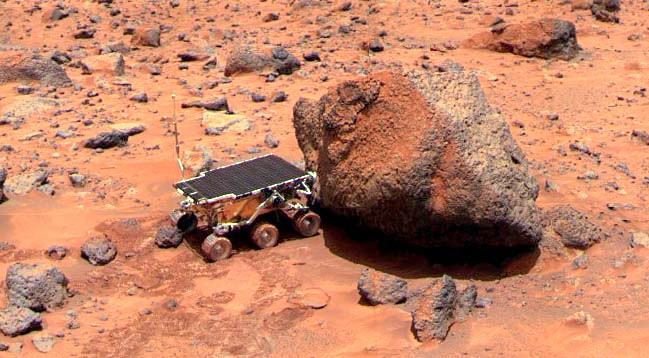
\includegraphics[width=0.8\textwidth]{img/Pathfinder01.jpg}
\end{center}
\end{frame}




\begin{frame}{Mars Pathfinder}
\large
A few days into the mission, the lander began experiencing resets. \\
\vspace{1em}
Data was being lost. \\
\vspace{1em}
The press reported these failures in terms such as ''software glitches'' and ''the computer was trying to do too many things at once''.
\end{frame}




\begin{frame}
\frametitle{Mars Pathfinder}
\large
Pathfinder contained an ``information bus''. \\
\vspace{1em}
A bus management task ran frequently with high priority to move certain kinds of data in and out. \\
\vspace{1em}
Access to the bus was synchronized with mutual exclusion locks. \\
\end{frame}




\begin{frame}
\frametitle{Mars Pathfinder}
The meteorological data gathering task ran as an infrequent, low priority task. \\
\vspace{1em}
When publishing, it would lock the bus, do writes to the bus, and then unlock it. \\
\vspace{1em}
The spacecraft also contained a communications task that ran with medium priority. \\
\vspace{1em}
If an interrupt caused the information bus thread to be scheduled while the bus was locked, the problem occurred. \\
\end{frame}




\begin{frame}{Mars Pathfinder}
Most of the time this combination worked fine.  \\
\vspace{1em}
It was possible for the communications task to be scheduled while the information bus task was waiting for the low priority task.\\
\vspace{1em}
The communications task, having higher priority, would prevent the lower priority meteorological task from running.\\
\quad... and therefore the information bus task could not run.
\end{frame}





\begin{frame}{Mars Pathfinder}
\large
After some time had passed, a watchdog timer would go off. \\
\vspace{1em}
The data bus task had not been executed for some time.  \\
\vspace{1em}
The watchdog concluded that something had gone drastically wrong, and initiated a total system reset.\\
\end{frame}



\section{Timer Coalescing}



\begin{frame}{Timer Coalescing}
\large
Using timers has an impact on power consumption.  \\
\vspace{1em}
Suppose an interval timer set up with an interval of 1000ms. \\
\vspace{1em}
Every second the system will execute the timer's action -- the system wakes up, runs the action, then goes back to sleep. \\
\end{frame}



\begin{frame}{Timer Coalescing}
\Large
What if there are multiple interval timers? \\
\vspace{1em}
The system might never actually get to sleep; \\
\quad constantly being woken up by interval timers.
\end{frame}




\begin{frame}
\frametitle{Timer Coalescing}
\begin{center}
	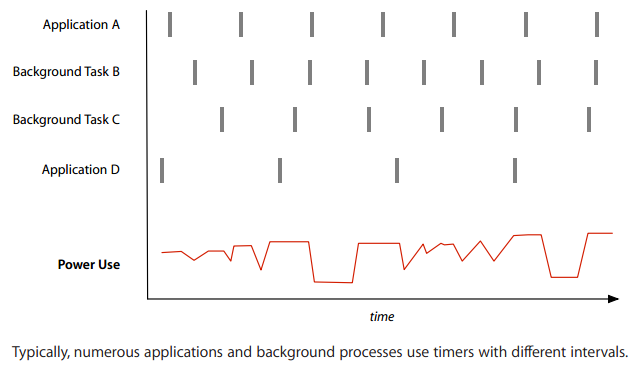
\includegraphics[width=0.85\textwidth]{img/coalesced_before.png}
\end{center}
\end{frame}





\begin{frame}
\frametitle{Timer Coalescing Semantics}
A critical insight about timers. \\
\vspace{1em}
For a 1000ms timer, the system does not promise that the timer will run exactly 1000 ms from now. \\
\vspace{1em}
What it really says is that the timer task will execute \alert{no sooner than} 1000 ms from now. \\
\vspace{1em}
It could be 1004 ms or 1200 ms later;\\
\quad yet it could not be 997 ms or 980 ms later.
\end{frame}




\begin{frame}{Timer Coalescing Semantics}
\Large
The OS can do something clever using these semantics. \\
\vspace{1em}
Delay some timers a little bit so that they line up.
\end{frame}




\begin{frame}
\frametitle{Timer Coalescing}
\begin{center}
	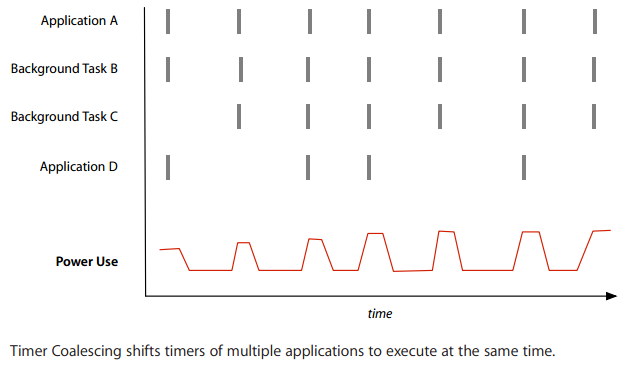
\includegraphics[width=0.85\textwidth]{img/coalesced-after.png}
\end{center}
\end{frame}




\begin{frame}{Timer Coalescing Semantics}
Now, this image is not a hundred percent accurate. \\
\vspace{1em}
Some of the lines were moved to the left (back in time) to make them line up. \mnote{and that would violate the no-sooner-than semantics.} \\
\vspace{1em}
This is just artistic license; in reality the lines could only be shifted to the right.\\
\vspace{1em} 
Most modern operating systems do this, including Windows and Mac OS X.\\
\end{frame}



\section*{Java Exceptions}



%%%%%%%%%%%%%%%%%%%%%%%%%%%%%%%%%%%%%%%%%%%%%%%%%%%%%%%%%%%%%%%%%%%%%%%%%%%%%%%%%%%%
% Exceptions
%%%%%%%%%%%%%%%%%%%%%%%%%%%%%%%%%%%%%%%%%%%%%%%%%%%%%%%%%%%%%%%%%%%%%%%%%%%%%%%%%%%%
\begin{frame}{Exceptions}
\texttt{Exception}s are used to signal an error (something unusual) during the execution of a program. \\
\vspace{1em}
This disrupts the normal flow of the program's instructions. \\
\vspace{1em}
An \texttt{Exception} is ``thrown'' when it is generated. \\
\vspace{1em}
The keyword is \texttt{throw}. \\
\end{frame}
%%%%%%%%%%%%%%%%%%%%%%%%%%%%%%%%%%%%%%%%%%%%%%%%%%%%%%%%%%%%%%%%%%%%%%%%%%%%%%%%%%%%



%%%%%%%%%%%%%%%%%%%%%%%%%%%%%%%%%%%%%%%%%%%%%%%%%%%%%%%%%%%%%%%%%%%%%%%%%%%%%%%%%%%%
% Exceptions
%%%%%%%%%%%%%%%%%%%%%%%%%%%%%%%%%%%%%%%%%%%%%%%%%%%%%%%%%%%%%%%%%%%%%%%%%%%%%%%%%%%%
\begin{frame}{Exceptions}
Exceptions are generated automatically or explicitly in a program.\\
\vspace{1em}
Write: \texttt{throw new RuntimeException(...)} \\
\vspace{1em}
The JRE may also generate an exception: \\
\vspace{1em}
Call \texttt{toString()} on an object that is null. JRE throws a \texttt{NullPointerException}. \\
\vspace{1em}
There are many different exceptions in Java (and you can make your own!). \\
\end{frame}
%%%%%%%%%%%%%%%%%%%%%%%%%%%%%%%%%%%%%%%%%%%%%%%%%%%%%%%%%%%%%%%%%%%%%%%%%%%%%%%%%%%%



%%%%%%%%%%%%%%%%%%%%%%%%%%%%%%%%%%%%%%%%%%%%%%%%%%%%%%%%%%%%%%%%%%%%%%%%%%%%%%%%%%%%
% Handling the Exception
%%%%%%%%%%%%%%%%%%%%%%%%%%%%%%%%%%%%%%%%%%%%%%%%%%%%%%%%%%%%%%%%%%%%%%%%%%%%%%%%%%%%
\begin{frame}{Handling the Exception}
If there is no code to ''handle'' an exception, then it goes up one level to the caller of that method until it gets to \texttt{main}. \\
\vspace{1em}
If \texttt{main} cannot deal with it either, then execution of the program will be stopped. \\
\vspace{1em}
An error message will be printed on the screen.  \\
\vspace{1em}
How to handle the exception? With an exception handler.  \\
\end{frame}
%%%%%%%%%%%%%%%%%%%%%%%%%%%%%%%%%%%%%%%%%%%%%%%%%%%%%%%%%%%%%%%%%%%%%%%%%%%%%%%%%%%%



%%%%%%%%%%%%%%%%%%%%%%%%%%%%%%%%%%%%%%%%%%%%%%%%%%%%%%%%%%%%%%%%%%%%%%%%%%%%%%%%%%%%
% Catching Exceptions
%%%%%%%%%%%%%%%%%%%%%%%%%%%%%%%%%%%%%%%%%%%%%%%%%%%%%%%%%%%%%%%%%%%%%%%%%%%%%%%%%%%%
\begin{frame}[fragile]{Catching Exceptions}
We place code that might throw an exception in a \texttt{try} block. \\
\vspace{1em}
Given that an \texttt{Exception} is \texttt{throw}n, it should come as no surprise that the keyword to handle it is \texttt{catch}. \\
\vspace{1em}
\begin{Verbatim}
try {
  // Some statements   
} catch (Exception e) {
  // Handle the Exception
}
\end{Verbatim}
\end{frame}
%%%%%%%%%%%%%%%%%%%%%%%%%%%%%%%%%%%%%%%%%%%%%%%%%%%%%%%%%%%%%%%%%%%%%%%%%%%%%%%%%%%%



%%%%%%%%%%%%%%%%%%%%%%%%%%%%%%%%%%%%%%%%%%%%%%%%%%%%%%%%%%%%%%%%%%%%%%%%%%%%%%%%%%%%
% Try-Catch Block
%%%%%%%%%%%%%%%%%%%%%%%%%%%%%%%%%%%%%%%%%%%%%%%%%%%%%%%%%%%%%%%%%%%%%%%%%%%%%%%%%%%%
\begin{frame}[fragile]{Try-Catch Block}
Let's look at an example:

\begin{Verbatim}
public void handleException() {
  Object example = null;
  try {
    System.out.println(example.toString());
  } catch (NullPointerException npe) {
    // Handle the NPE
  }
}
\end{Verbatim}
\end{frame}
%%%%%%%%%%%%%%%%%%%%%%%%%%%%%%%%%%%%%%%%%%%%%%%%%%%%%%%%%%%%%%%%%%%%%%%%%%%%%%%%%%%%



%%%%%%%%%%%%%%%%%%%%%%%%%%%%%%%%%%%%%%%%%%%%%%%%%%%%%%%%%%%%%%%%%%%%%%%%%%%%%%%%%%%%
% Dealing with the Exception
%%%%%%%%%%%%%%%%%%%%%%%%%%%%%%%%%%%%%%%%%%%%%%%%%%%%%%%%%%%%%%%%%%%%%%%%%%%%%%%%%%%%
\begin{frame}{Dealing with the Exception}
\large
How we handle an exception depends on the exception and the specific program. \\ 
\vspace{1em}
Sometimes you might just display an error message. \\
\vspace{1em}
In some cases you don't even want to handle the error. \\
\vspace{1em}
Maybe the output contains information to find the problem. \\
\end{frame}
%%%%%%%%%%%%%%%%%%%%%%%%%%%%%%%%%%%%%%%%%%%%%%%%%%%%%%%%%%%%%%%%%%%%%%%%%%%%%%%%%%%%



%%%%%%%%%%%%%%%%%%%%%%%%%%%%%%%%%%%%%%%%%%%%%%%%%%%%%%%%%%%%%%%%%%%%%%%%%%%%%%%%%%%%
% Multiple Catch Blocks
%%%%%%%%%%%%%%%%%%%%%%%%%%%%%%%%%%%%%%%%%%%%%%%%%%%%%%%%%%%%%%%%%%%%%%%%%%%%%%%%%%%%
\begin{frame}[fragile]{Multiple Catch Blocks}
\begin{Verbatim}
try {
  // Some statements   
} catch (NullPointerException e) {
  // Handle the Exception
} catch (IOException e2) {
  // Do Something Else
} catch (FileNotFoundException | SQLException e3) {
  // Some other things
}
\end{Verbatim}
\end{frame}
%%%%%%%%%%%%%%%%%%%%%%%%%%%%%%%%%%%%%%%%%%%%%%%%%%%%%%%%%%%%%%%%%%%%%%%%%%%%%%%%%%%%



%%%%%%%%%%%%%%%%%%%%%%%%%%%%%%%%%%%%%%%%%%%%%%%%%%%%%%%%%%%%%%%%%%%%%%%%%%%%%%%%%%%%
% The Finally Block
%%%%%%%%%%%%%%%%%%%%%%%%%%%%%%%%%%%%%%%%%%%%%%%%%%%%%%%%%%%%%%%%%%%%%%%%%%%%%%%%%%%%
\begin{frame}{The Finally Block}
\large
Optionally, after the catch block: the \texttt{finally} block.  \\
\vspace{1em}
The finally block always executes when the try block exits, whether it went to the catch block or not.  \\
\vspace{1em}
Use: avoid having cleanup code accidentally bypassed by a \texttt{return}, \texttt{continue}, or \texttt{break}.\\
\end{frame}
%%%%%%%%%%%%%%%%%%%%%%%%%%%%%%%%%%%%%%%%%%%%%%%%%%%%%%%%%%%%%%%%%%%%%%%%%%%%%%%%%%%%



%%%%%%%%%%%%%%%%%%%%%%%%%%%%%%%%%%%%%%%%%%%%%%%%%%%%%%%%%%%%%%%%%%%%%%%%%%%%%%%%%%%%
% Finally Block Format
%%%%%%%%%%%%%%%%%%%%%%%%%%%%%%%%%%%%%%%%%%%%%%%%%%%%%%%%%%%%%%%%%%%%%%%%%%%%%%%%%%%%
\begin{frame}[fragile]{Try-Catch-Finally}
\begin{Verbatim}
try {
  // Some statements   
} catch (Exception e) {
  // Handle the Exception
} finally {
  // Cleanup
}
\end{Verbatim}
\end{frame}
%%%%%%%%%%%%%%%%%%%%%%%%%%%%%%%%%%%%%%%%%%%%%%%%%%%%%%%%%%%%%%%%%%%%%%%%%%%%%%%%%%%%



%%%%%%%%%%%%%%%%%%%%%%%%%%%%%%%%%%%%%%%%%%%%%%%%%%%%%%%%%%%%%%%%%%%%%%%%%%%%%%%%%%%%
% Finally Blocks
%%%%%%%%%%%%%%%%%%%%%%%%%%%%%%%%%%%%%%%%%%%%%%%%%%%%%%%%%%%%%%%%%%%%%%%%%%%%%%%%%%%%
\begin{frame}[fragile]{Finally Blocks}
What is the return value of this function?

\begin{Verbatim}
public boolean tryFinally() {
  try {
    return false;
  } finally {
    return true;
  }
}
\end{Verbatim}
\end{frame}
%%%%%%%%%%%%%%%%%%%%%%%%%%%%%%%%%%%%%%%%%%%%%%%%%%%%%%%%%%%%%%%%%%%%%%%%%%%%%%%%%%%%



%%%%%%%%%%%%%%%%%%%%%%%%%%%%%%%%%%%%%%%%%%%%%%%%%%%%%%%%%%%%%%%%%%%%%%%%%%%%%%%%%%%%
% Exceptions: Putting it Together
%%%%%%%%%%%%%%%%%%%%%%%%%%%%%%%%%%%%%%%%%%%%%%%%%%%%%%%%%%%%%%%%%%%%%%%%%%%%%%%%%%%%
\begin{frame}[fragile]{Exceptions: Putting it Together}
\Large
Let's see a simple example of our new exception handling knowledge.
\end{frame}
%%%%%%%%%%%%%%%%%%%%%%%%%%%%%%%%%%%%%%%%%%%%%%%%%%%%%%%%%%%%%%%%%%%%%%%%%%%%%%%%%%%%




%%%%%%%%%%%%%%%%%%%%%%%%%%%%%%%%%%%%%%%%%%%%%%%%%%%%%%%%%%%%%%%%%%%%%%%%%%%%%%%%%%%%
% Exception Handling
%%%%%%%%%%%%%%%%%%%%%%%%%%%%%%%%%%%%%%%%%%%%%%%%%%%%%%%%%%%%%%%%%%%%%%%%%%%%%%%%%%%%
\begin{frame}{Exception Handling}
Sometimes we don't want to handle an exception ourselves; sometimes we want to ``pass the buck''.  \\
\vspace{1em}
To do that, declare that your method \texttt{throws} an exception: \\
\vspace{1em}
\texttt{public void writeList() throws IOException}. \\
\vspace{1em}
Then handling the \texttt{IOException} is the responsibility of whatever method calls \texttt{writeList()}. \\
\end{frame}
%%%%%%%%%%%%%%%%%%%%%%%%%%%%%%%%%%%%%%%%%%%%%%%%%%%%%%%%%%%%%%%%%%%%%%%%%%%%%%%%%%%%



%%%%%%%%%%%%%%%%%%%%%%%%%%%%%%%%%%%%%%%%%%%%%%%%%%%%%%%%%%%%%%%%%%%%%%%%%%%%%%%%%%%%
% Creating Exceptions
%%%%%%%%%%%%%%%%%%%%%%%%%%%%%%%%%%%%%%%%%%%%%%%%%%%%%%%%%%%%%%%%%%%%%%%%%%%%%%%%%%%%
\begin{frame}{Creating Exceptions}
\Large
Want to create an exception in your code?  \\
\vspace{0.5em}
Use the \texttt{throw} keyword.  \\
\vspace{0.5em}
\texttt{throw new RunTimeException()} \\
\vspace{0.5em}
Throw whatever type of exception is appropriate. \\
\end{frame}
%%%%%%%%%%%%%%%%%%%%%%%%%%%%%%%%%%%%%%%%%%%%%%%%%%%%%%%%%%%%%%%%%%%%%%%%%%%%%%%%%%%%



%%%%%%%%%%%%%%%%%%%%%%%%%%%%%%%%%%%%%%%%%%%%%%%%%%%%%%%%%%%%%%%%%%%%%%%%%%%%%%%%%%%%
% Final Thoughts on Exceptions
%%%%%%%%%%%%%%%%%%%%%%%%%%%%%%%%%%%%%%%%%%%%%%%%%%%%%%%%%%%%%%%%%%%%%%%%%%%%%%%%%%%%
\begin{frame}{Final Thoughts on Exceptions}
\Large
As a final note, exceptions are supposed to be exceptional. \\
\vspace{1em}
Don't use them as part of the expected flow of your program. \\
\vspace{1em}
Use them to handle error conditions \& unexpected situations. \\
\end{frame}
%%%%%%%%%%%%%%%%%%%%%%%%%%%%%%%%%%%%%%%%%%%%%%%%%%%%%%%%%%%%%%%%%%%%%%%%%%%%%%%%%%%%



\end{document}